\documentclass{ximera}
\usepackage[colorlinks=true,urlcolor=blue]{hyperref}
\title{What is Ximera?}
\begin{document}
\begin{abstract}
An introduction to the Ximera system.
\end{abstract}
\maketitle

\href{http://ximera.osu.edu}{\sf Ximera}
is an open-source software project that
seeks to help course instructors create learning materials
for their students both as PDF files and as webpages
simultaneously. Our strategy to achieve this goal is to separate
content from deployment.

An author writes content in a \LaTeX\ document.
As usual this produces a PDF file that can be distributed to students.
Next the author communicates this file to
\href{http://github.com}{\tt github.com},
a free web-based service providing a number of features to authors.
This causes the
\href{http://ximera.osu.edu}{\sf Ximera}
interpreter to post the file in the form of an interactive webpage
that students can access.
This process is illustrated in the figure below.

\begin{image}
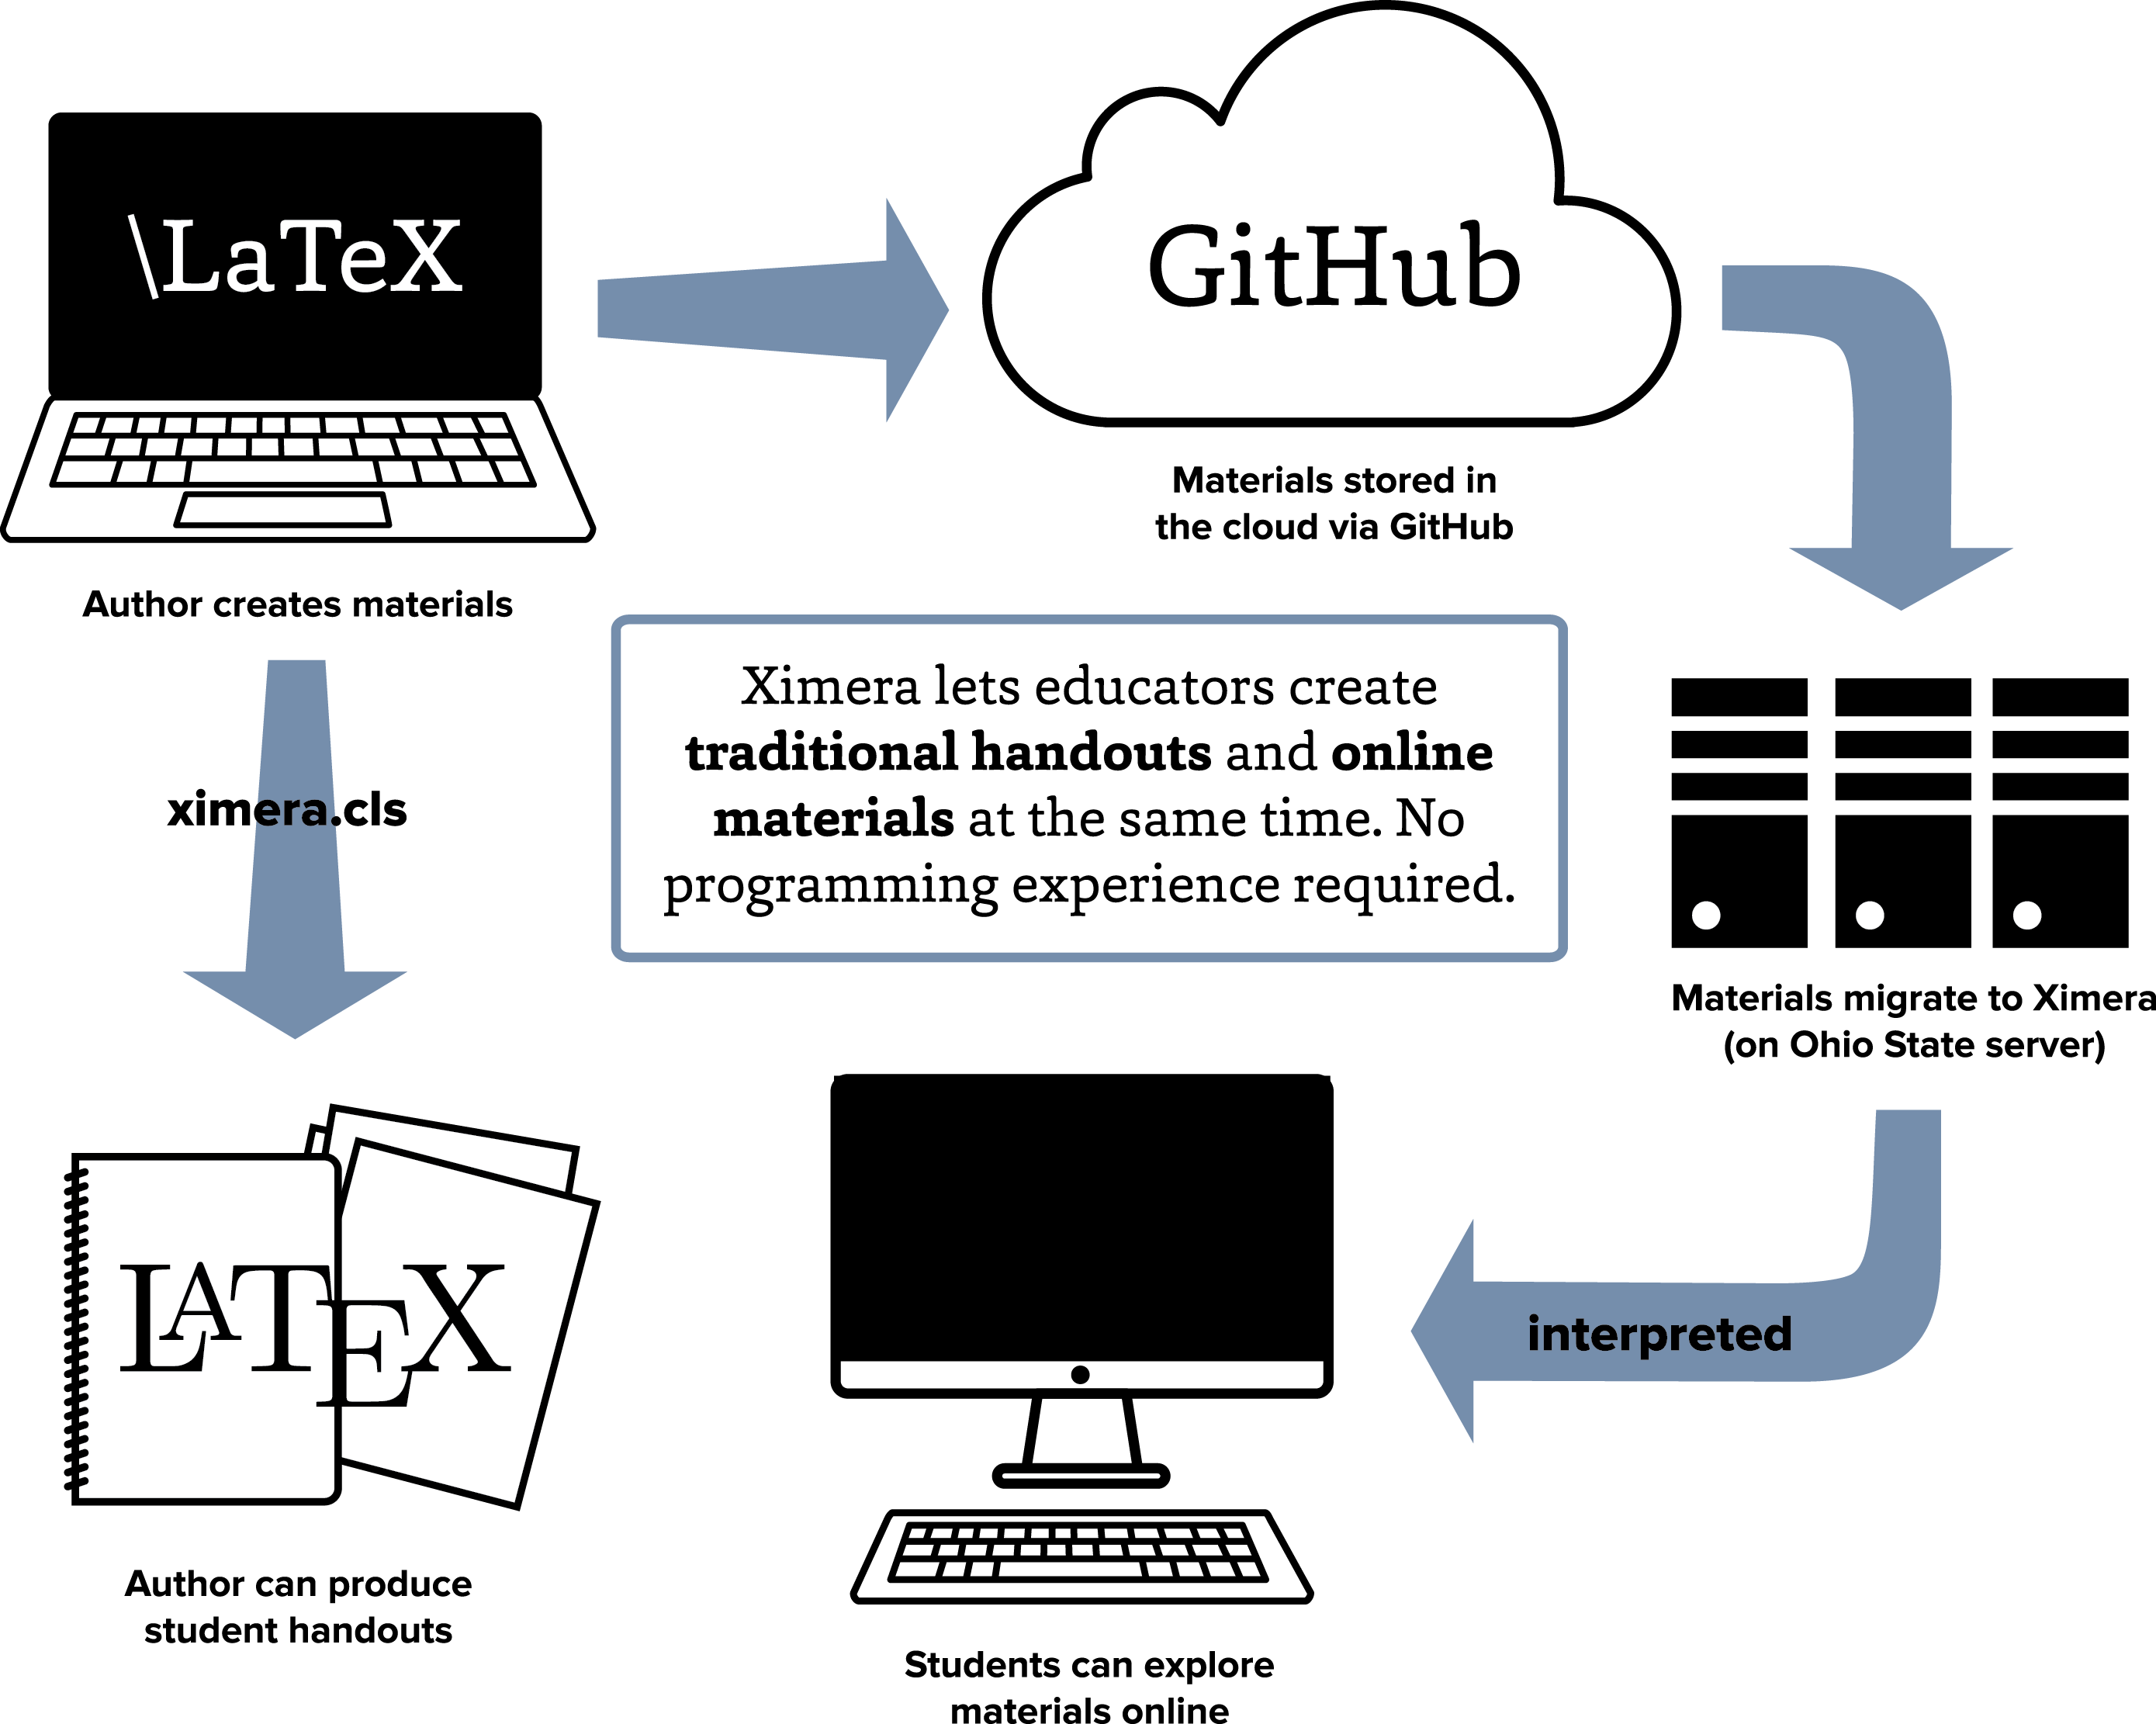
\includegraphics[scale=.5]{XimeraGraphic.png}
\end{image}

\end{document}
